\documentclass[twocolumn]{article}
\usepackage{fullpage}
\usepackage{amssymb}
\usepackage{amsmath}
\usepackage{enumerate}
\usepackage{graphicx}
\usepackage[margin=2.2cm]{geometry}

\newcommand{\RR}{\mathbb{R}}
\newcommand{\ra}{\rightarrow}
\newcommand{\Wo}{W^{(1)}}
\newcommand{\Wt}{W^{(2)}}
\newcommand{\bo}{b^{(1)}}
\newcommand{\bt}{b^{(2)}}
\newcommand{\xii}{x^{(i)}}

\title{Properties of Autoencoders}
\author{%\sectionsize
    Justin Johnson \\
    \texttt{jcjohns@stanford.edu}
  \and
    Bharath Ramsundar \\
    \texttt{rbharath@stanford.edu}
}
\date{}

\begin{document}

\maketitle

% \section{Introduction}
% Some recent applications of deep learning have utilized unsupervised pretraining to greatly improve
% their performance on classification tasks \cite{le2011building}. One of the fundamental building
% blocks of unsupervised pretraining is the sparse autoencoder. In this project we aim to develop a
% theoretical and practical understanding of different varieties of autoencoders.
% 
% \vspace{-1pc}
% 
% \section{Definitions}
% A single-layer autoencoder is a neural network with a single hidden layer that attempts to learn
% the identity function. The hidden layer activations of a trained autoencoder can then be used as a
% feature vector for the original data.
% 
% More precisely, let $\Wo\in\RR^{p\times n}$ and $\Wt\in\RR^{n\times p}$ be matrices of
% weights, let $\bo\in\RR^p$ and $\bt\in\RR^n$ be bias vectors, and let $f:\RR\ra\RR$ be
% an activation function; a common choice is the sigmoid $f(z)=1/(1+e^{-z})$. These parameters
% define a neural network with a single hidden layer. For an input $x\in\RR^n$ the output of the
% network is $h_{W,b}(x)=f(\Wt f(\Wo x+\bo)+\bt)$ where $f$ is applied componentwise.
% The term $f(\Wo x+\bo)$ represents the activations of the input $x$ on the hidden layer of the
% network. To train an autoencoder, we are given data $x^{(1)},\ldots,x^{(m)}\in\RR^n$ and we must find
% $W$ and $b$ to minimize the reconstruction error $\sum_i\|h_{W,b}(\xii)-\xii\|$ under some norm;
% additional constraints such as regularization or sparsity may also be imposed.
% 
% A sparse autoencoder imposes additional constraints on the hidden layer activations averaged over
% the training data which is given by $\hat\rho=\frac1m\sum_if(\Wo\xii+\bo)$. Typically we want to force
% $\hat\rho$ to be close to some desired activation level $\rho$.
% 
% \section{Connection to PCA}
% If we only attempt to minimize the $\ell^2$ reconstruction error $\sum_i\|h_{W,b}(\xii)-\xii\|$
% then the features learned by the single layer autoencoder are closely related to the principal
% components of the training data\cite{bourlard1988auto}. More specifically, let $X\in\RR^{n\times m}$
% be a matrix whose $i$th column is $\xii$. Let $H=f(\Wt X+\bo u^T)$ where $u\in\RR^m$ has $u_i=1$
% for all $i$. Then $H$ gives the hidden layer activations of all training data points.
% If $\hat W$ and $\hat b$ are the optimal choices of the parameters and $\hat H$ is the hidden layer
% activations of the training data for these optimal parameters then it can be shown that
% $\hat\Wt\hat H$ is the optimal rank $p$ approximation to the mean-subtracted training data
% $X'=X-Xuu^T/n$ which can be calculated using the singular value decomposition of $X'$.
% A similar result can also be shown for multi-layered autoencoders.
% 
% This shows that an autoencoder that only minimizes $\ell^2$ reconstruction error essentially does
% nothing more than compute the principal components of the training data. This suggests that the
% relative success of autoencoders in recent years is most likely due to the additional sparsity constraint.
% 
% \section{Linearization}
% We considered a linearization of a neural net. That is, we defined the transfer function
% $f$ to be the identity function. Then $h_{W,b}(x) =W^{(2)}(W^{(1)}x + b^{(1)}) + b^{(2)}$.
% % We can rewrite this as $h_{W,b}(x)
% % = W^{(2)}W^{(1)} x + b$. To simplify the problem, we constrain $W^{(2)} =
% % (W^{(1)})^T$ and $b = 0$. Let $W = W^{(1)}$. Then $h_{W,b}(x) = W^TW x$.
% We also add a $\ell^2$ sparsity constraint $\|\rho - \hat{\rho}\|_2^2$. The minimization problem then becomes
% \[\min_{W,b} \sum_{i=1}^m \|h_{W,b}(\xii) - \xii\|_2^2  + \beta \|\rho - \hat{\rho}\|_2^2\]
% We explicitly derived the gradient of the above formula and implemented gradient descent.
% 
% \section{Future Work}
% In the reminder of this project, we will explore the effects of various
% regularization and sparsity constraints on the neural network. We will also
% consider whether higher order Taylor approximations to nonlinear neural nets
% work better in practice than our linear models. Our goal is to build intuition
% about how the various components of neural networks affect performance in hopes
% of eventually proving nontrivial theoretical bounds.
% 
% \pagebreak

\section{Introduction}
In recent years a variety of deep learning algorithms, including deep belief networks
\cite{hinton2006fast,lee2009convolutional} and deep neural networks, both convolutional
\cite{krizhevsky2012imagenet} and non-convolutional \cite{le2011building}. The types of
networks that are typically used in these applications are very complicated, and studying
their theoretical properties is very difficult.

Some approaches have utilized unsupervised
pretraining of deep neural networks in order to improve performance on classification tasks
\cite{le2011building}. One of the fundamental building blocks of this unsupervised pretraining
process is the sparse autoencoder. A single-layer autoencoder is a much simpler object than
an entire deep network, but even this relatively simple object has not been well-studied
theoretically.

In this project we aim to explore different varieties of autoencoders and to try and understand
why they work.

\vspace{-0.5pc}
\section{Sparse Autoencoder}
A sparse autoencoder is a neural network with a single hidden layer that attempts to learn the
identity function. The transfer function in these networks is nonlinear; in our experiments we use
the sigmoid transfer function $f(z)=1/(1+e^{-z})$.

Neural net weights are learned by minimizing an objective function consisting
of three terms. The first term is the $\ell^2$ reconstruction error of the training data.
The second term is $\ell^2$ regularization of the weight vectors. The third term constrains the
mean activation of each hidden layer neuron over the training set. The sparsity constraint can take
many forms, but our initial implementation uses a penalty of the form 
\[\sum_{j=1}^p\left(\rho\log\frac{\rho}{\hat\rho_j}+(1-\rho)\log\frac{1-\rho}{1-\hat\rho_j}\right)\]
where the hidden layer contains $p$ neurons, $\hat\rho_j$ is the mean activation of the $j$th hidden
layer neuron over the training set, and $\rho$ is a constant controlling the desired sparsity.
The weights of the trained network can be viewed as a feature transform for the training data.
We implemented this algorithm and ran it on the MNIST dataset \cite{lecun1998mnist}; the learned
feature transform is shown in Figure~\ref{fig:features}. Qualitatively, the learned features
roughly correspond to local object parts.

\vspace{-1.1pc}
\section{Equivalence with PCA}
An autoencoder that does not include the regularization or sparsity terms learns a feature
representation that is closely related to the principal components of the training data
\cite{bourlard1988auto}. We implemented this type of autoencoder on the MNIST dataset and
also ran principal component analysis on the same dataset; the learned features can be seen
in Figure~\ref{fig:features}. The learned features appear to be qualitatively similar.

This equivalence between ``vanilla'' autoencoders and principal component analysis suggests
that the recent success of autoencoders is due to the additional constraints placed upon
their parameters. This motivates a more in-depth analysis of the sparsity constraint.

\vspace{-1pc}
\section{Sparse Linear Autoencoders}
We next considered a sparse linearized autoencoder where the transfer function is simply the identity
function. The objective function for this autoencoder is the sum of the $\ell^2$ reconstruction error,
an $\ell^2$ regularization term on the network weights, and an $\ell^2$ sparsity constraint of the form
$\|\rho-\hat\rho\|_2^2$ where as above $\hat\rho_j$ is the mean activation of the $j$th hidden unit
on the training set. The learned features for this autoencoder is shown in Figure~\ref{fig:features}.

\section{Discussion}
Our experimentation so far has led us to focus on the sparsity constraint of the autoencoder.
For the remainder of the term we will consider other variants on this constraint both on
nonlinear and linearized networks. In particular, we will experiment with $\ell^1$ and $\ell^2$
sparsity constraints on the nonlinear network and an $\ell^1$ sparsity constraint on the
linearized network. Depending on the results of these experiments, we will attempt to understand
the theoretical implications of these sorts of constraints. In addition to the linearized
autoencoder, we would also like to experiment with networks whose transfer function is a Taylor
approximation to the sigmoid function.

\begin{figure*}
  \centering
  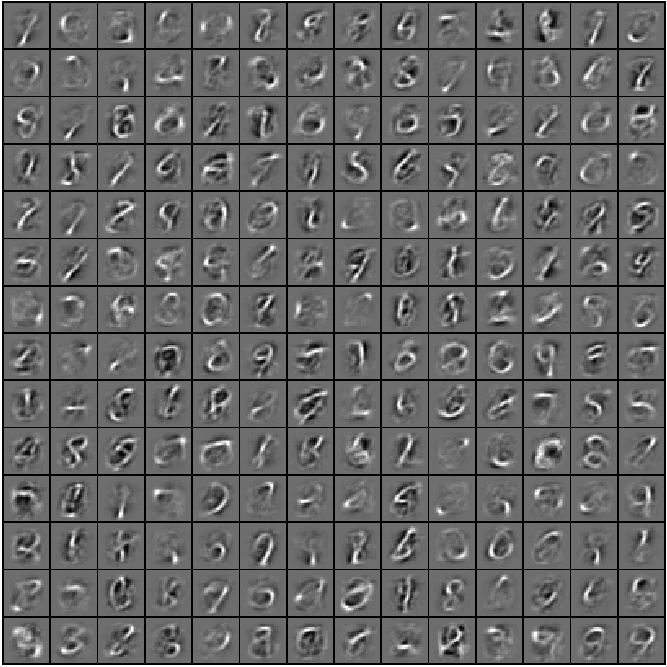
\includegraphics[width=0.45\textwidth]{sparsesigmoidnn.png}
  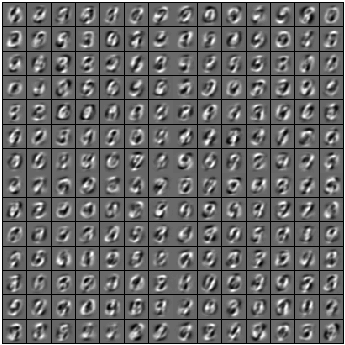
\includegraphics[width=0.45\textwidth]{linearnn.png}
  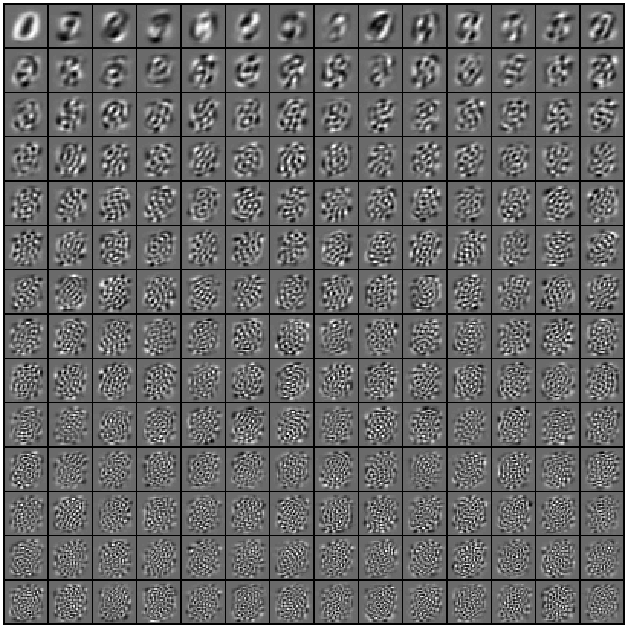
\includegraphics[width=0.45\textwidth]{pca.png}
  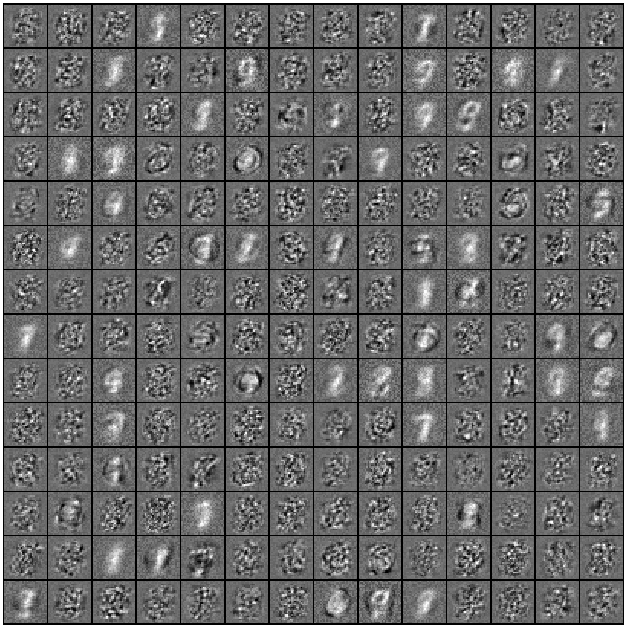
\includegraphics[width=0.45\textwidth]{nonlinearnn.png}
  \caption{Learned features for MNIST using different methods.
      Upper left: Sparse (nonlinear) autoencoder.
      Upper right: Sparse linear autoencoder.
      Lower left: Principal component analysis.
      Lower right: nonlinear autoencoder.
    }
  \label{fig:features}
\end{figure*}

\bibliographystyle{plain}
\bibliography{refs}

\end{document}
